\section{Handling Distortion}

When constructing our camera model in section \ref{sec:camera_model}, we made the assumption that the camera we are using can be approximated using a pinhole camera.


Modern cameras rarely have a single lens. Rather, they typically have compound lens




\subsection{Symmetrical Radial Distortion}

Symmetrical lens distortion refers to

It


\begin{figure}[H]
    \centering
    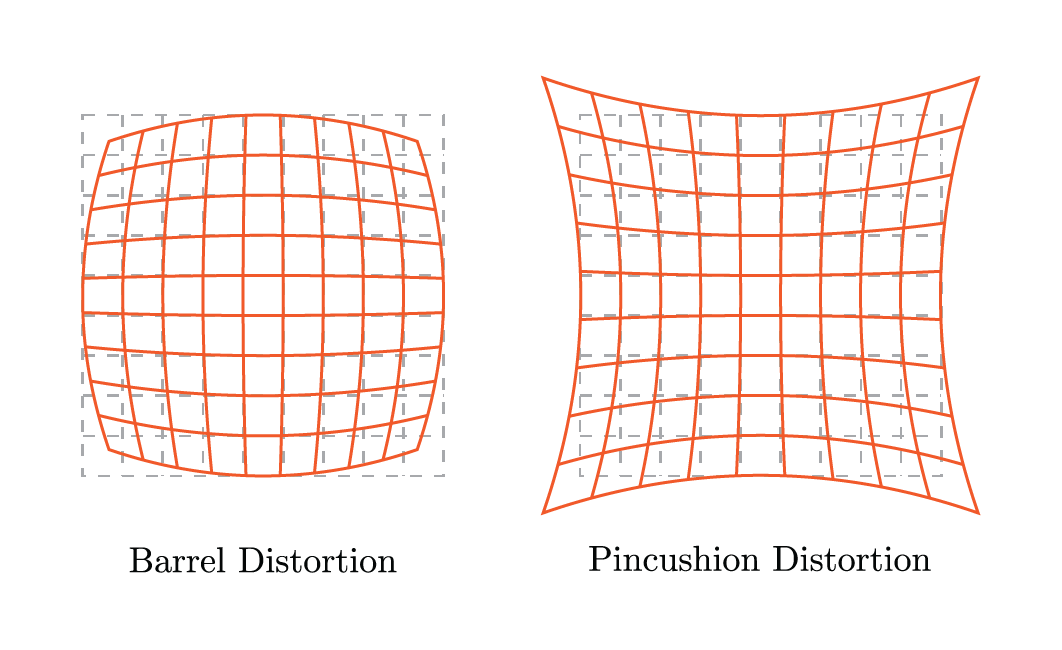
\includegraphics[width=0.9\textwidth]{images/radial_distortion}
    \caption{Types of radial distortion.}
\end{figure}

\subsection{Asymmetrical Radial Distortion}

\subsection{Tangential (Decentering) Distortion}

of axis

\begin{figure}[H]
    \centering
    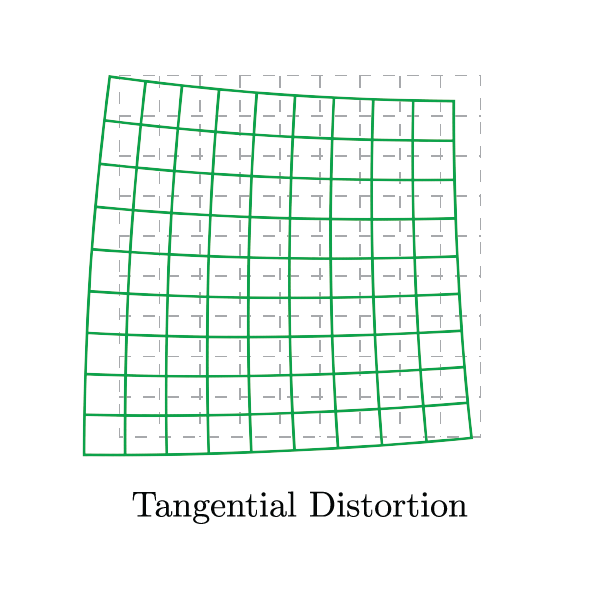
\includegraphics[width=0.45\textwidth]{images/tangential_distortion}
    \caption{Tangential (Decentering) Distortion}
\end{figure}

\begin{figure}[H]
    \centering
    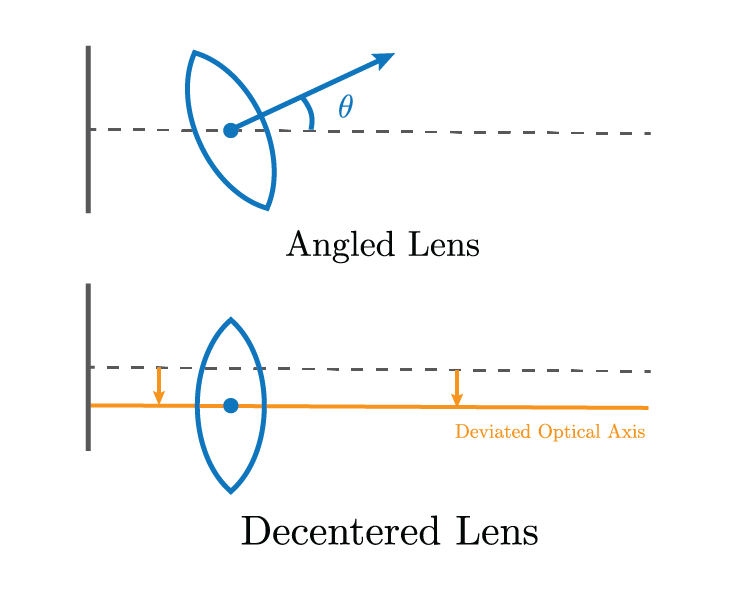
\includegraphics[width=0.5\textwidth]{figures/lens_alignment}
    \caption{Reasons why tangential distortion can occur}
\end{figure}

\subsection{Brown-Conrady Model}
